%----------------------------------------------------------------------------------------
%	PACKAGES AND OTHER DOCUMENT CONFIGURATIONS
%----------------------------------------------------------------------------------------
% \documentclass[12pt,a4paper]{article}
\documentclass[paper=a4, fontsize=11pt]{scrartcl} % A4 paper and 11pt font size

%\usepackage[T1]{fontenc} % Use 8-bit encoding that has 256 glyphs
%\usepackage{fourier} % Use the Adobe Utopia font for the document - comment this line to return to the LaTeX default

%%% Работа с русским языком
\usepackage{cmap}					% поиск в PDF
\usepackage{mathtext} 				% русские буквы в фомулах
\usepackage[T2A]{fontenc}			% кодировка
\usepackage[utf8]{inputenc}			% кодировка исходного текста
\usepackage[english,russian]{babel}	% локализация и переносы

% Работа с графикой
\usepackage{graphicx}
\graphicspath{{images/}{images/png/}}
\usepackage{wrapfig}
\setlength{\intextsep}{5pt plus 1.0pt minus 1.0pt}
\usepackage{movie15}
\usepackage{media9}
\usepackage{animate}
\usepackage{hyperref}
\usepackage{subcaption}

\makeatletter
\setlength{\@fptop}{0pt}
\setlength{\@fpbot}{0pt plus 1fil}
\makeatother

\renewcommand{\topfraction}{1}
\renewcommand{\textfraction}{0}

\usepackage{sectsty} % Allows customizing section commands
\allsectionsfont{\centering \normalfont\scshape} % Make all sections centered, the default font and small caps

\usepackage{fancyhdr} % Custom headers and footers
\pagestyle{fancyplain} % Makes all pages in the document conform to the custom headers and footers
\fancyhead{} % No page header - if you want one, create it in the same way as the footers below
\fancyfoot[L]{} % Empty left footer
\fancyfoot[C]{} % Empty center footer
\fancyfoot[R]{\thepage} % Page numbering for right footer
\renewcommand{\headrulewidth}{0pt} % Remove header underlines
\renewcommand{\footrulewidth}{0pt} % Remove footer underlines
\setlength{\headheight}{10.6pt} % Customize the height of the header


\usepackage{amsmath}
\numberwithin{equation}{section} % Number equations within sections (i.e. 1.1, 1.2, 2.1, 2.2 instead of 1, 2, 3, 4)
\numberwithin{figure}{section} % Number figures within sections (i.e. 1.1, 1.2, 2.1, 2.2 instead of 1, 2, 3, 4)
\numberwithin{table}{section} % Number tables within sections (i.e. 1.1, 1.2, 2.1, 2.2 instead of 1, 2, 3, 4)
\DeclareMathOperator*{\argmax}{arg\,max}

\setlength\parindent{0pt} % Removes all indentation from paragraphs - comment this line for an assignment with lots of text


\usepackage{enumerate}

%----------------------------------------------------------------------------------------
%	TITLE SECTION
%----------------------------------------------------------------------------------------

\newcommand{\horrule}[1]{\rule{\linewidth}{#1}} % Create horizontal rule command with 1 argument of height
\newcommand{\No}{\textnumero} % символ номера №

\title{	
	\huge Подготовка к экзамену по нейронным сетям \\ % The assignment title
	\horrule{2pt} \\[0.5cm] % Thick bottom horizontal rule
}

\author{Клочков Вадим} % Your name
\date{}


\begin{document}
	
	\maketitle % Print the title
	
	%----------------------------------------------------------------------------------------
	%	PROBLEM 1
	%----------------------------------------------------------------------------------------
	\section{Нейронные сети прямого распространения(feed forward neural networks, FFNN) и перцептроны}
	FFNN сети передают информацию от входа к выходу. Нейроны одного слоя не связаны между собой, а соседние слои обычно полностью связаны. \\
	Самая простая нейронная сеть имеет два входных нейрона и один выходной, и может использоваться в качестве модели логических вентилей. FFNN обычно получает множества входных и выходных данных. Этот процесс называется обучением с учителем. Обучение обычно происходит по методу обратного распространения ошибки. Данная ошибка является разницей между вводом и выводом.
	
	Перцептрон.
	
	\begin{figure}[h!]
		\centering
		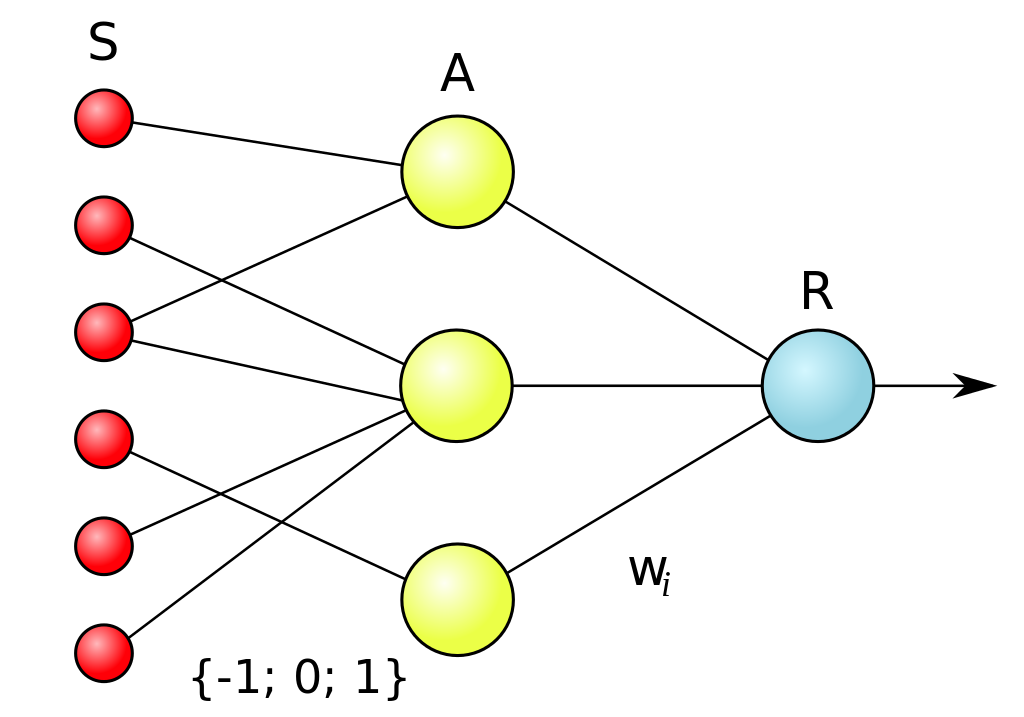
\includegraphics[scale=0.25]{perc}
	\end{figure}

	Элементарный перцептрон состоит из элементов трёх типов: $S$-элементов, $A$-элементов и одного $R$-элемента. \\
	$S$-элементы — это слой сенсоров или рецепторов(т.е. входной слой). Каждый рецептор может находиться в одном из двух состояний — покоя или возбуждения, и только в последнем случае он передаёт единичный сигнал в следующий слой, ассоциативным элементам.
	
	$A$-элементы называются ассоциативными, потому что каждому такому элементу, как правило, соответствует целый набор (ассоциация) $S$-элементов. $A$-элемент активизируется, как только количество сигналов от $S$-элементов на его входе превысило некоторую величину $\theta$.
	
	Сигналы от возбудившихся $A$-элементов, в свою очередь, передаются в сумматор $R$, причём сигнал от $i$-го ассоциативного элемента передаётся с коэффициентом $w_{i}$. Этот коэффициент называется весом $A-R$ связи.
	
	Так же как и $A$-элементы, $R$-элемент подсчитывает сумму значений входных сигналов, помноженных на веса. $R$-элемент, а вместе с ним и элементарный перцептрон, выдаёт $1$, если линейная форма превышает порог $\theta$, иначе на выходе будет $-1$.
	
	Обучение элементарного перцептрона состоит в изменении весовых коэффициентов $w_{i}$ связей $A-R$. После обучения перцептрон готов работать в режиме распознавания или обобщения.
	
	
	\begin{figure}[h!]
		\centering
		\begin{subfigure}[b]{0.3\textwidth}
			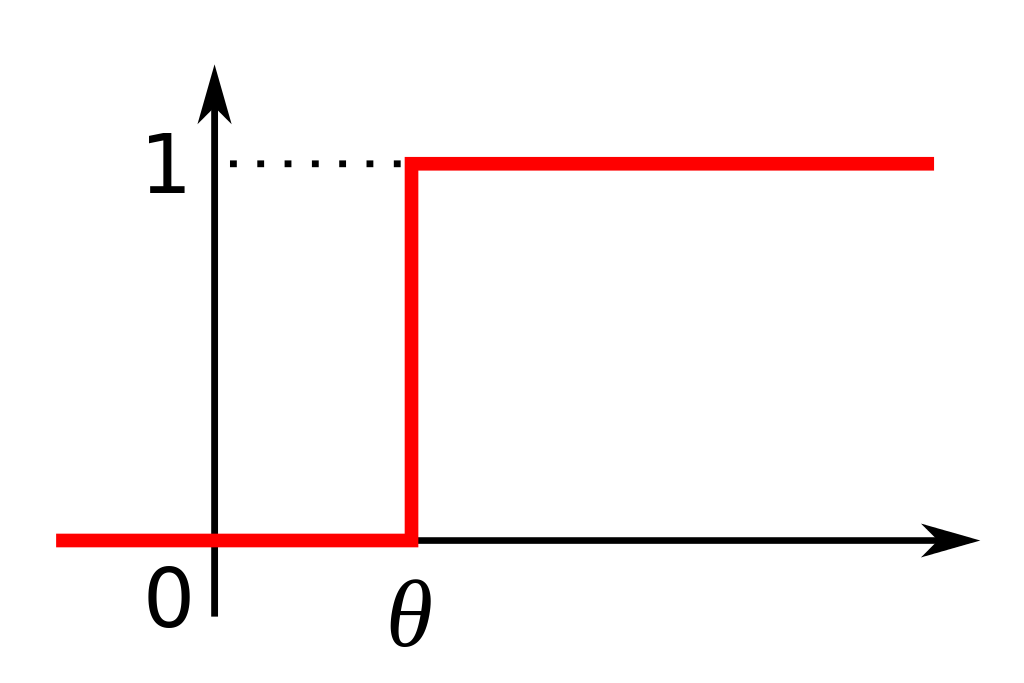
\includegraphics[width=\textwidth]{S-A}
			\caption{Пороговая функция, реализуемая простыми S- и A-элементами.}
		\end{subfigure}
		\begin{subfigure}[b]{0.3\textwidth}
			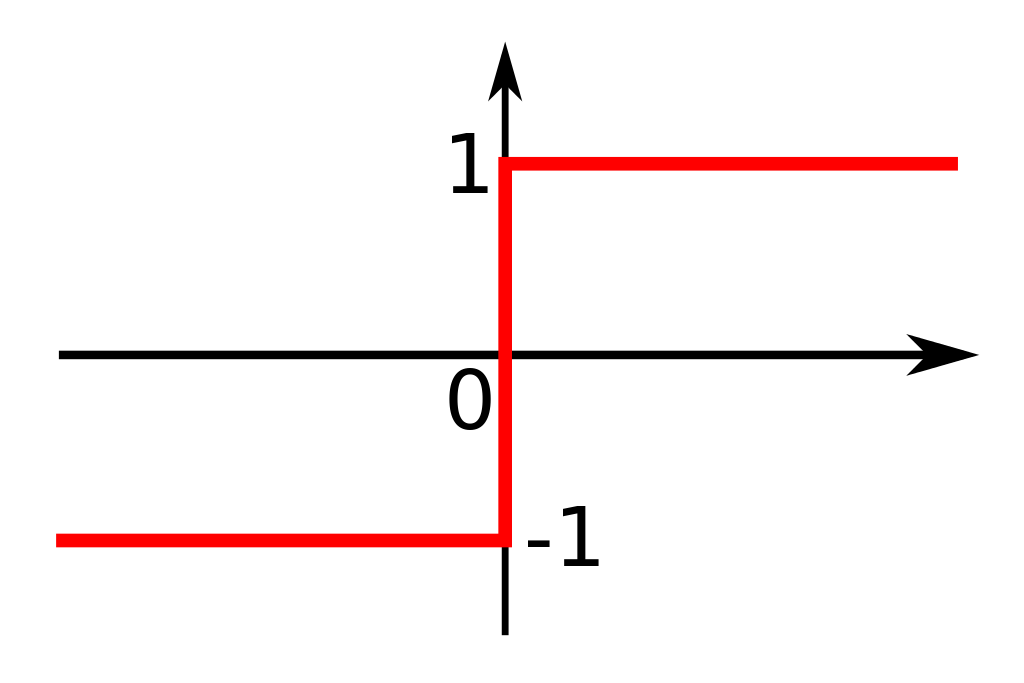
\includegraphics[width=\textwidth]{R}
			\caption{Пороговая функция, реализуемая простым R-элементом.}
		\end{subfigure}

	\end{figure}

	\begin{enumerate}
	\item \textbf{Перцептрон} представляет собой сеть, состоящую из $S-$, $A-$, $R-$элементов, с переменной матрицей взаимодействия $W$ (элементы которой $w_{ij}$ — весовые коэффициенты), определяемой последовательностью прошлых состояний активности сети.
	\item \textbf{Простым} перцептроном называется любая система, удовлетворяющая следующим условиям:
	\begin{enumerate}	
		\item в системе имеется только один $R-$элемент (естественно, он связан всеми $A-$элементами)
		\item система представляет собой перцептрон с последовательными связями, идущими только от $S-$элементов к $A-$элементам и от $A-$элементов к $R-$элементам
		\item веса всех связей от $S-$элементов к $A-$элементам ($S-A$ связей) неизменны
		\item все активирующие функции $S-$, $A-$, $R-$элементов имеют вид $U_{i}(t)=f(a_{i}(t))$, где $a_{i}(t)$ - алгебраическая сумма всех сигналов, поступающих одновременно на вход элемента $u_{i}$
	\end{enumerate}
	\item \textbf{Элементарным} перцептроном называется простой перцептрон, у которого все элементы - простые. В этом случае его активизирующая функция имеет вид $c_{ij}(t)=U_{i}(t-\tau )w_{ij}(t)$
	\end{enumerate}

	\textbf{Многослойный перцептрон}\\
	(по Розенблатту) - это перцептрон, в котором присутствуют дополнительные слои $A-$элементов.\\
	(по Румельхарту) - это перцептрон, в котором присутствуют дополнительные слои $A-$элементов, причём, обучение такой сети проводится по методу обратного распространения ошибки, и обучаемыми являются все слои перцептрона (в том числе $S-A$). Является частным случаем многослойного перцептрона Розенблатта.
	
	\begin{figure}[h!]
		\centering
		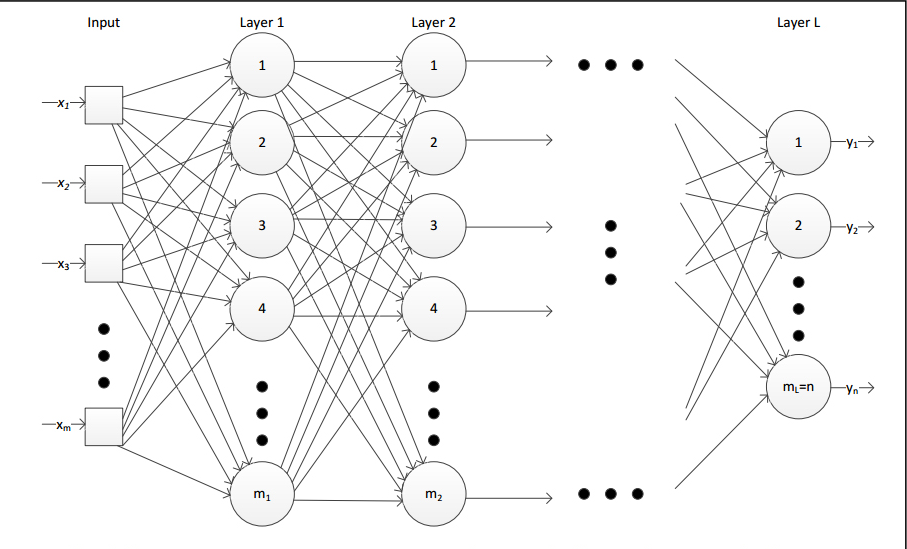
\includegraphics[scale=0.45]{mlp}
	\end{figure}
	
	\textbf{Обучение перцептрона}\\
	Классический метод обучения перцептрона — это метод коррекции ошибки.\\
	Допустим, мы хотим обучить перцептрон разделять два класса объектов. Для этого выполним следующий алгоритм:
	
	\begin{enumerate}	
		\item Случайным образом выбираем пороги для $A-$элементов и устанавливаем связи $S-A$ (далее они изменяться не будут).
		\item Начальные коэффициенты $w_{i}$ полагаем равными нулю.
		\item Предъявляем обучающую выборку: объекты (например, круги либо квадраты) с указанием класса, к которым они принадлежат.
		\begin{enumerate}	
			\item Показываем перцептрону объект первого класса. При этом некоторые $A-$элементы возбудятся. Коэффициенты $w_{i}$, соответствующие этим возбуждённым элементам, увеличиваем.
			\item Предъявляем объект второго класса и коэффициенты $w_{i}$ тех $A-$элементов, которые возбудятся при этом показе, уменьшаем.
		\end{enumerate}
		\item Обе части шага 3 выполним для всей обучающей выборки. В результате обучения сформируются значения весов связей $w_{i}$.
	\end{enumerate}

	\textbf{More information(можно пропустить)}
	Теорема сходимости перцептрона, описанная и доказанная Ф. Розенблаттом, показывает, что элементарный перцептрон, обучаемый по такому алгоритму, независимо от начального состояния весовых коэффициентов и последовательности появления стимулов всегда приведёт к достижению решения за конечный промежуток времени.

	%----------------------------------------------------------------------------------------
	%	PROBLEM 2
	%----------------------------------------------------------------------------------------
	\section{Сети радиально-базисных функций}
	
	Сети радиально-базисных функций (radial basis function, RBF) — это FFNN, которая содержит промежуточный (скрытый) слой радиально симметричных нейронов. Такой нейрон преобразовывает расстояние от данного входного вектора до соответствующего ему "центра" по некоторому нелинейному закону.
	
	Радиальная функция — это функция $f(x)$, зависящая только от расстояния между $x$ и фиксированной точкой пространства $X$. 
	
	Основное свойство радиально-симметричных функций – это монотонное и симметричное относительно некоторой вертикальной оси симметрии изменение (убывание или возрастание) их откликов.
	
	В качестве примера такой функции может служить выражение функции Гаусса. Именно эта функция наиболее часто используется в рассматриваемой архитектуре нейронных сетей, однако главным образом, в ее многомерном случае:
	$$h(x) = exp(\frac{(\|x - \vec{c}\|)^2}{r^2}),$$
	где $\vec{c}$ вектор центров (координат вертикальных осей симметрии) множества радиально-симметричных функций;  $\|x - \vec{c}\|$ норма вектора отклонений входной переменной от центров радиально-симметричных функций.
	
	
	%----------------------------------------------------------------------------------------
	%	PROBLEM 3
	%----------------------------------------------------------------------------------------
	\section{Нейронная сеть Хопфилда(Hopfield network, HN) }
	Нейронная сеть Хопфилда — полносвязная нейронная сеть с симметричной матрицей связей. В процессе работы динамика таких сетей сходится к одному из положений равновесия. Эти положения равновесия определяются заранее в процессе обучения. \\
	Такая сеть может быть использована как автоассоциативная память, как фильтр, а также для решения некоторых задач оптимизации. В отличие от многих нейронных сетей, работающих до получения ответа через определённое количество тактов, сети Хопфилда работают до достижения равновесия, когда следующее состояние сети в точности равно предыдущему: начальное состояние является входным образом, а при равновесии получают выходной образ.
	
	Нейронная сеть Хопфилда устроена так, что её отклик на запомненные $m$ эталонных «образов» составляют сами эти образы, а если образ немного исказить и подать на вход, он будет восстановлен и в виде отклика будет получен оригинальный образ. Таким образом, сеть Хопфилда осуществляет коррекцию ошибок и помех.
	
	Матрица весов $W$ определяется один раз и в последствии не меняется. Пусть $x_1, x_2, \ldots x_n$ - входные образы, которые мы запоминаем. Тогда
	$$W = \sum_{k = 1}^{M} x_k^T \cdot x_k$$
	Образ $x_i$ - это вектор размера $n$, где $n$ - кол-во входов нашей сети.
	
	Пусть мы имеем на вход некий вектор $y$, который не похож ни на один из $x_i$. Т.е. имеем поврежденный/зашумленный сигнал. Для распознавания таких сигналов и используется сеть Хопфилда. 
	
	Наш вектор $y$ умножается на веса $W$. Назовем полученный вектор $y*$. Далее применяем функцию активации $f$. Результат после применения функции активации - $y'$ подаем на вход. Данный алгоритм действует до тех пор, пока $y'$ не будет равен одному из образов $x_i$. 
	
	Существует 2 типа сети: синхронная и асинхронная. Синхронной называют ту, где на вход мы подаем весь вектор $y'$, а асинхронной ту, где подаем вектор, часть которого состоит из исходного $y$, а часть из $y'$.
	
	\begin{figure}[h!]
		\centering
		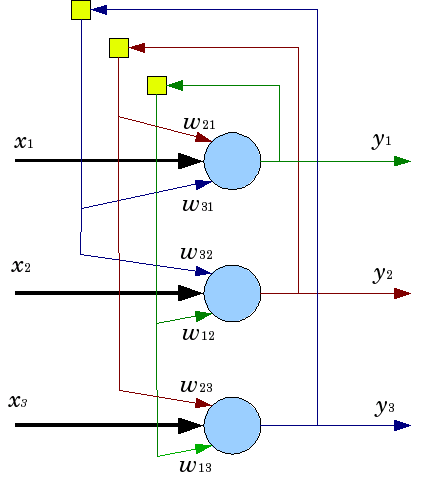
\includegraphics[scale=0.45]{Hopfield's_net}
	\end{figure}
	
	%----------------------------------------------------------------------------------------
	%	PROBLEM 4
	%----------------------------------------------------------------------------------------
	\section{Цепи Маркова (Markov chains, MC или discrete time Markov Chains, DTMC)}
	Цепи Маркова — это предшественники машин Больцмана (BM) и сетей Хопфилда (HN). Их смысл можно объяснить так: каковы мои шансы попасть в один из следующих узлов, если я нахожусь в данном? Каждое следующее состояние зависит только от предыдущего. Хотя на самом деле цепи Маркова не являются НС, они весьма похожи. Также цепи Маркова не обязательно полносвязны.
	
	Все состояния можно описать вершинами графа. Например, такими вершинами могут быть положения человека: [лежит], [сидит], [стоит], [идет]
	
	\begin{figure}[h!]
		\centering
		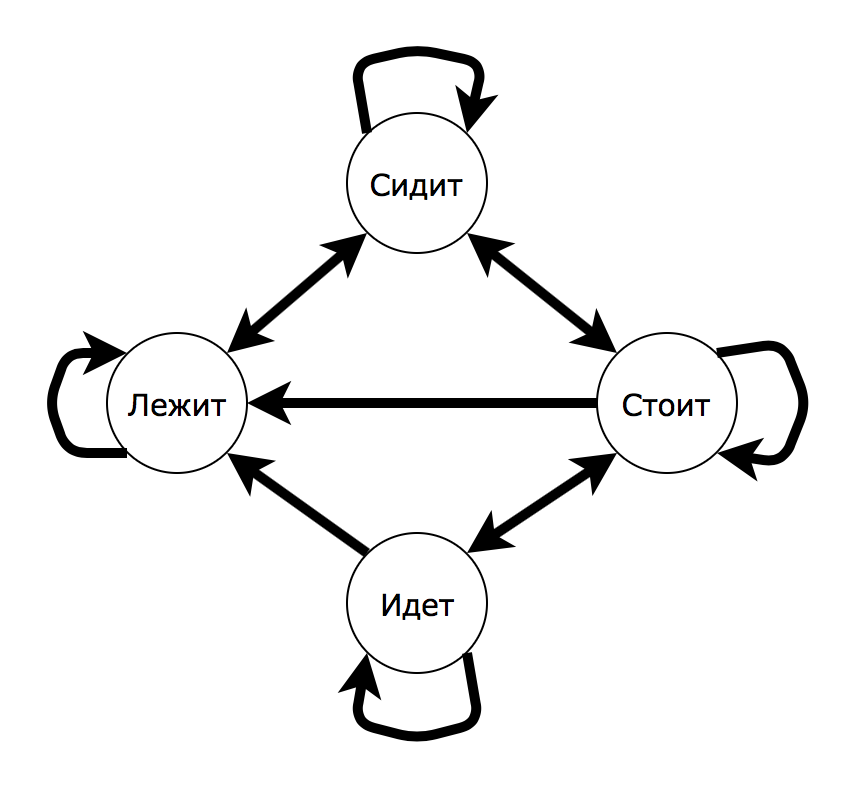
\includegraphics[scale=0.25]{graph}
	\end{figure}
	
	Здесь видно, что граф ориентированный, это значит, что не из всякого состояния можно попасть в другое. Например, если вы лежите, то невозможно сразу пойти. Нудно сначала сесть, потом встать, а только потом пойти. Но упасть и оказаться лежачим можно из любого положения ))  \\
	Каждая связь имеет некую вероятность. Так, например, вероятность упасть из стоячего положения очень маленькая, гораздо вероятнее стоять дальше, пойти или сесть. Сумма всех вероятностей равна 1.
	
	Кроме всего прочего цепи Маркова позволяют генерировать события. 
	
	%----------------------------------------------------------------------------------------
	%	PROBLEM 5
	%----------------------------------------------------------------------------------------
	\section{Машина Больцмана (Boltzmann machine, BM)}
	Машина Больцмана — это стохастическая сеть. Обучение проходит по методу обратного распространения ошибки или по алгоритму сравнительной расходимости.  В целом процесс обучения очень похож на таковой у сети Хопфилда.
	Некоторые нейроны помечены как входные, а некоторые — как скрытые.
	
	\begin{figure}[h!]
		\centering
		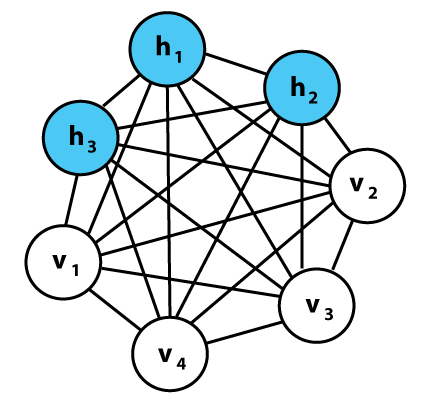
\includegraphics[scale=0.45]{Boltzmannexamplev1}
	\end{figure}
	
	
	%----------------------------------------------------------------------------------------
	%	PROBLEM 6
	%----------------------------------------------------------------------------------------
	\section{Ограниченная машина Больцмана(restricted Boltzmann machine, RBM)}
	Ограниченная машина Больцмана - вид генеративной стохастической нейронной сети, которая определяет распределение вероятности на входных образцах данных.
	Она очень похожа на машину Больцмана. Единственной разницей является её ограниченность. В ней нейроны одного типа не связаны между собой.
	
	\begin{figure}[h!]
		\centering
		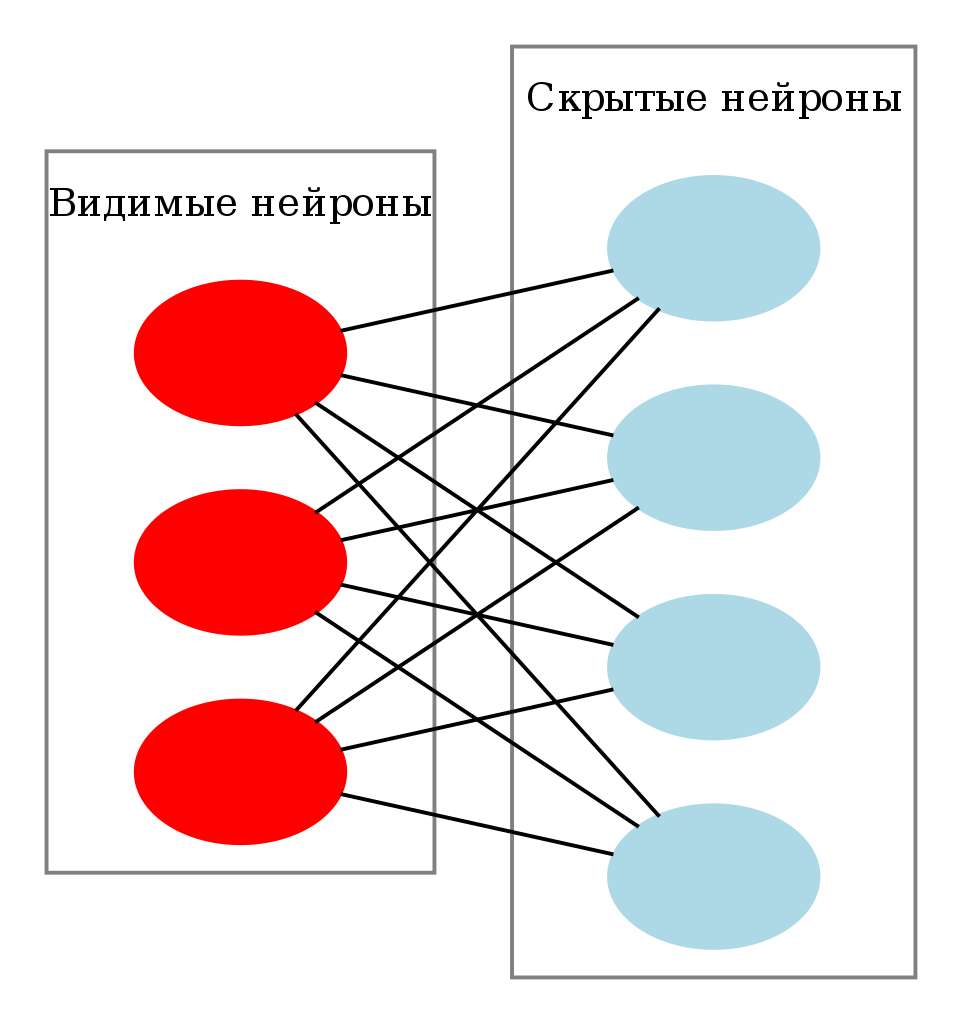
\includegraphics[scale=0.18]{Restricted_Boltzmann_machine}
	\end{figure}
	
	Особенностью ограниченных машин Больцмана является возможнность проходить обучение без учителя.
	Ограниченные машины Больцмана имеют широкий спектр применений - это задачи снижения размерности данных, задачи классификации, коллаборативная фильтрация(Коллаборативная фильтрация — это один из методов построения прогнозов (рекомендаций) в рекомендательных системах, использующий известные предпочтения группы пользователей для прогнозирования неизвестных предпочтений другого пользователя), выделение признаков (feature learning) и тематическое моделирование(Тематическое моделирование — способ построения модели коллекции текстовых документов, которая определяет, к каким темам относится каждый из документов).
	
	В ограниченной машине Больцмана нейроны образуют двудольный граф. Такая система связей позволяет применить при обучении сети метод градиентного спуска с контрастивной дивергенцией.
	
	\subsection{Алгоритм обучения}
	Целью обучения является максимизация вероятности системы с заданным набором образцов $V$ (матрицы,в которой каждая строка соответствует одному образцу видимого вектора $v$), определяемой как произведение вероятностей: $$\argmax_W \prod\limits_{v \in V} P(v)$$.
	
	Для тренировки нейронной сети используется алгоритм контрастивной дивергенции (CD) с целью нахождения оптимальных весов матрицы $W$. Алгоритм использует Семплирование по Гиббсу для организации процедуры градиентного спуска, аналогично методу обратного распространения ошибок для нейронных сетей.
	
	В целом один шаг контрастивной дивергенции (CD-1) выглядит следующим образом:
	\begin{enumerate}
		\item Для одного образца данных $v$ вычисляются вероятности скрытых элементов, и применяется активация для скрытого слоя $h$ для данного распределения вероятностей.
		\item Вычисляется внешнее произведение (семплирование) для $v$ и $h$, которое называют позитивным градиентом.
		\item Через образец $h$ проводится реконструкция образца видимого слоя $v'$, а потом выполняется снова семплирование с активацией скрытого слоя $h'$. (Этот шаг называется Семплирование по Гиббсу).
		\item Далее вычисляется внешнее произведение, но уже векторов $v'$ и $h'$, которое называют негативным градиентом.
		\item Матрица весов $W$ поправляется на разность позитивного и негативного градиента, помноженного на множитель, задающий скорость обучения: $\Delta W = \epsilon(vh^T - v'h'^T)$
	\end{enumerate}
	
	%----------------------------------------------------------------------------------------
	%	PROBLEM 7
	%----------------------------------------------------------------------------------------
	\section{Сеть типа «deep belief» (deep belief networks, DBN)}
	
	Сети глубинного доверия(Deep Belief Network) - это тип нейронных сетей, состоящих из нейскольких слоев скрытых переменных, с связами только между различными слоями. Сеть глубоко доверия можно обучить восстанавливать свои входные данные. Используется обучение без учителя. В дальнейшем такая сеть может быть обучена на размеченных данных для выполнения классификации.\\
	Сеть глубоко обучения также можно рассматривать как композицию простых сетей, таких как ограниченные машины Больцмана, в которых каждый слой(в том числе и скрытые слои), кроме последнего, служат входным для следующего
	слоя. Это дает возможность использовать быстрое послойное обучение нейросети, используя контрастивное расхождение(contrastive divergence), начиная с первых двух слоев.\\
	Так же есть наблюдение, сделанное Yee-Whye Teh, учеником Джеффри Хинтона, которое говорит о том, что DBN может быть обучена способом жадного послойного обучения.
	
	
	
	%----------------------------------------------------------------------------------------
	%	PROBLEM 8
	%----------------------------------------------------------------------------------------
	\section{Свёрточные нейронные сети и глубинные свёрточные нейронные сети}
	
	 В компьютерном зрении достаточно давно анализ изображений основан на применении фильтров — специальных преобразований, позволяющих обнаружить участки, обладающие определёнными свойствами. Примером может служить лапласовский фильтр, детектирующий края объектов на изображении. Позже возникла идея обучения фильтров под конкретную задачу, которая, в свою очередь, привела к появлению свёрточных слоёв и свёрточных нейронных сетей (convolutional neural networks).
	 
	\subsection{Структура}
	Что конкретно делают СНС? Берётся изображение, пропускается через серию свёрточных, нелинейных слоев, слоев объединения и полносвязных слоёв, и генерируется вывод. Выводом может быть класс или вероятность классов, которые лучше всего описывают изображение.

	Первые два типа слоев (convolutional, subsampling), чередуясь между собой, формируют входной вектор признаков для многослойного персептрона.
	
	\begin{figure}[h!]
		\center{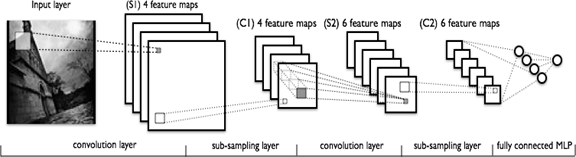
\includegraphics[scale=0.7]{struct}}
		\caption{Топология сверточной нейронной сети}
	\end{figure}

	\begin{figure}[h!]
		Так же возможна следующая конфигурация СНС:
		$$Input->Conv->ReLU->Conv->ReLU->Pool->...->Full\: Connected$$
	\end{figure}
	
	
	\subsection{Сверточный слой}
	Сверточный слой представляет из себя набор карт (другое название – карты признаков, в обиходе это обычные матрицы), у каждой карты есть синаптическое ядро (в разных источниках его называют по-разному: сканирующее ядро или фильтр). 
	\begin{wrapfigure}{r}{7cm}
		\centering
		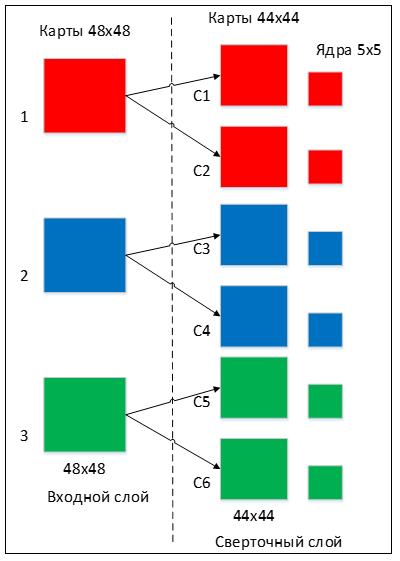
\includegraphics[scale=0.2]{karts}
		\caption{Организация связей}
	\end{wrapfigure}
	Количество карт определяется требованиями к задаче, если взять большое количество карт, то повысится качество распознавания, но увеличится вычислительная сложность. 
	В большинстве случаев предлагается брать соотношение один к двум, то есть каждая карта предыдущего слоя (например, у первого сверточного слоя, предыдущим является входной) связана с двумя картами сверточного слоя. Ядро представляет из себя фильтр или окно, которое скользит по всей области предыдущей карты и находит определенные признаки объектов. Например, если сеть обучали на множестве лиц, то одно из ядер могло бы в процессе обучения выдавать наибольший сигнал в области глаза, рта, брови или носа, другое ядро могло бы выявлять другие признаки. Размер ядра обычно берут в пределах от 3х3 до 7х7. Если размер ядра маленький, то оно не сможет выделить какие-либо признаки, если слишком большое, то увеличивается количество связей между нейронами. Также размер ядра выбирается таким, чтобы размер карт сверточного слоя был четным, это позволяет не терять информацию при уменьшении размерности в подвыборочном слое, описанном ниже. 
	
	Скажем, наш фильтр $ 7 \times 7 \times 1$, и он будет детектором кривых.
	
	\begin{figure}[h!]
		\center{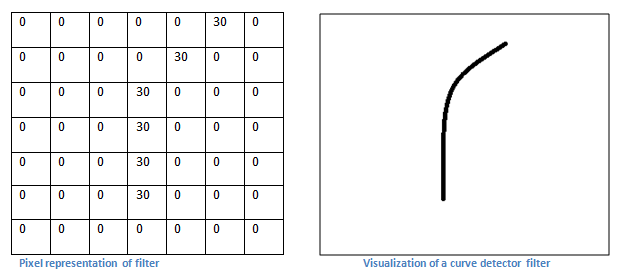
\includegraphics[scale=0.5]{filter1}}
	\end{figure}

	\begin{figure}[h!]
		Когда у нас в левом верхнем углу вводного изображения есть фильтр, он производит умножение значений фильтра на значения пикселей этой области. Давайте рассмотрим пример изображения, которому мы хотим присвоить класс, и установим фильтр в верхнем левом углу.
	\end{figure}

	

	\begin{figure}[h!]
		\center{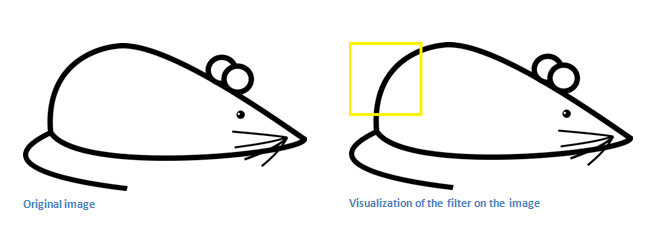
\includegraphics[scale=0.5]{filter2}}
	\end{figure}

	\begin{figure}[h!]
		Всё что нам нужно, это умножить значения фильтра на исходные значения пикселей изображения.
	\end{figure}
	

	\begin{figure}[h!]
		\center{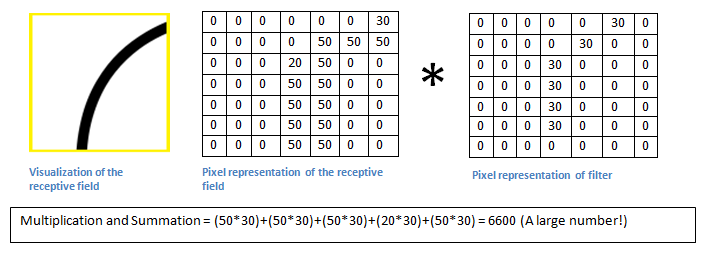
\includegraphics[scale=0.5]{filter3}}
	\end{figure}

	\begin{figure}[h!]
			По сути, если на вводном изображении есть форма, в общих чертах похожая на кривую, которую представляет этот фильтр, и все умноженные значения суммируются, то результатом будет большое значение! Теперь переместим фильтр.
	\end{figure}



	\begin{figure}[h!]
		\center{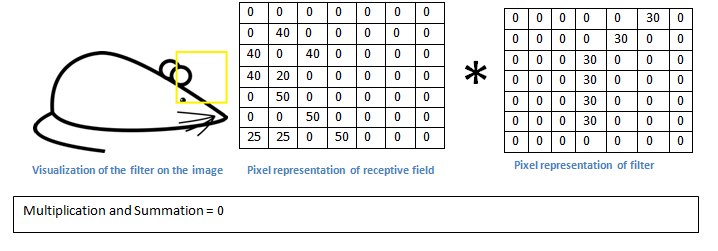
\includegraphics[scale=0.5]{filter4}}
	\end{figure}

	\begin{figure}[h!]
		Значение намного меньше. Это потому, что в новой области изображения нет ничего, что фильтр определения кривой мог засечь. Помните, что вывод этого свёрточного слоя — карта свойств. В самом простом случае, при наличии одного фильтра свертки (и если этот фильтр — детектор кривой), карта свойств покажет области, в которых больше вероятности наличия кривых.
		
		Вот еще несколько изображений для лучшего понимания:
	\end{figure}

	
	
	\begin{figure}[!h]
		\center{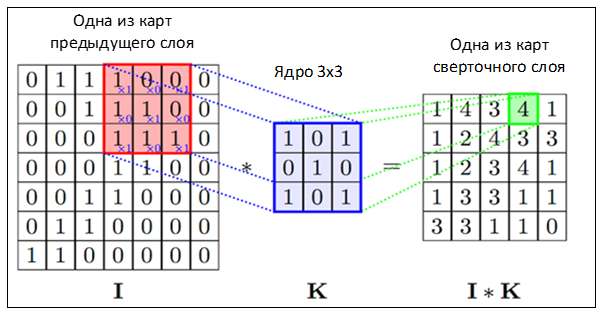
\includegraphics[scale=0.5]{filter5}}
	\end{figure}

	\begin{figure}[!h]
			При этом в зависимости от метода обработки краев исходной матрицы результат может быть меньше исходного изображения (valid), такого же размера (same) или большего размера (full)
	\end{figure}


	\begin{figure}[h!]
		\center{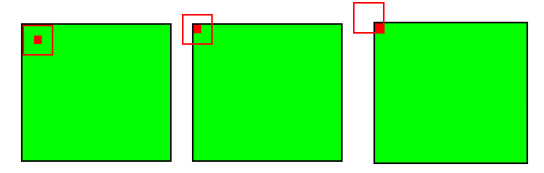
\includegraphics[scale=0.5]{filter6}}
	\end{figure}
	
	\begin{figure}[h!]
		\begin{frame}{Операция свертки. Ядро смещено, новая карта получается того же размера, что и предыдущая}
			\centering
			\animategraphics[loop,autoplay,width=0.5\linewidth]{0.8}{tmp-}{0}{45}
		\end{frame}
	\end{figure}
	
	\subsection{Подвыборочный слой(subsampling)}
	
	Цель слоя – уменьшение размерности карт предыдущего слоя. Если на предыдущей операции свертки уже были выявлены некоторые признаки, то для дальнейшей обработки настолько подробное изображение уже не нужно, и оно уплотняется до менее подробного. К тому же фильтрация уже ненужных деталей помогает не переобучаться. В процессе сканирования ядром подвыборочного слоя (фильтром) карты предыдущего слоя, сканирующее ядро не пересекается в отличие от сверточного слоя. Обычно, каждая карта имеет ядро размером 2x2, что позволяет уменьшить предыдущие карты сверточного слоя в 2 раза. Вся карта признаков разделяется на ячейки 2х2 элемента.
	Обычно в подвыборочном слое применяется функция активации ReLU. Операция подвыборки (или MaxPooling – выбор максимального) 
	
	\begin{figure}[h]
		\centering
		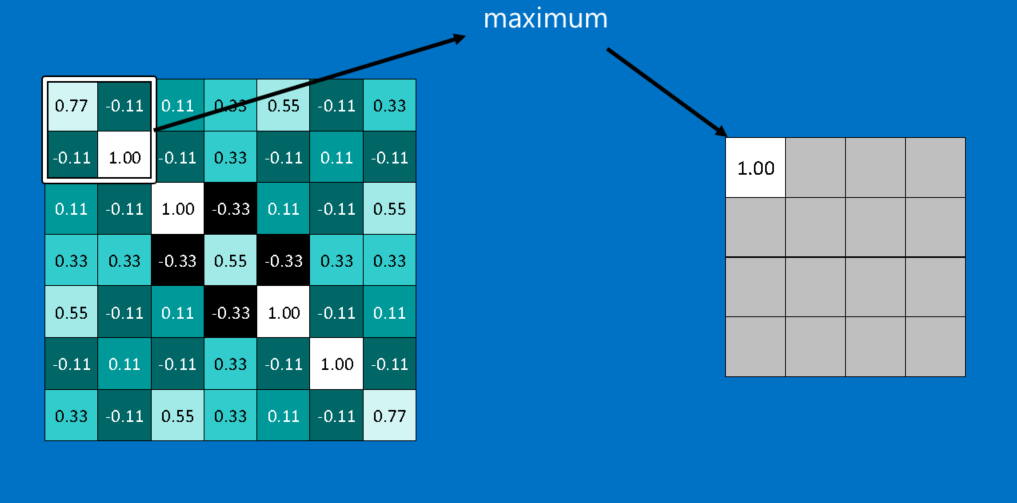
\includegraphics[scale=0.5]{pool}
	\end{figure}

	\begin{figure}[h]
		\centering
		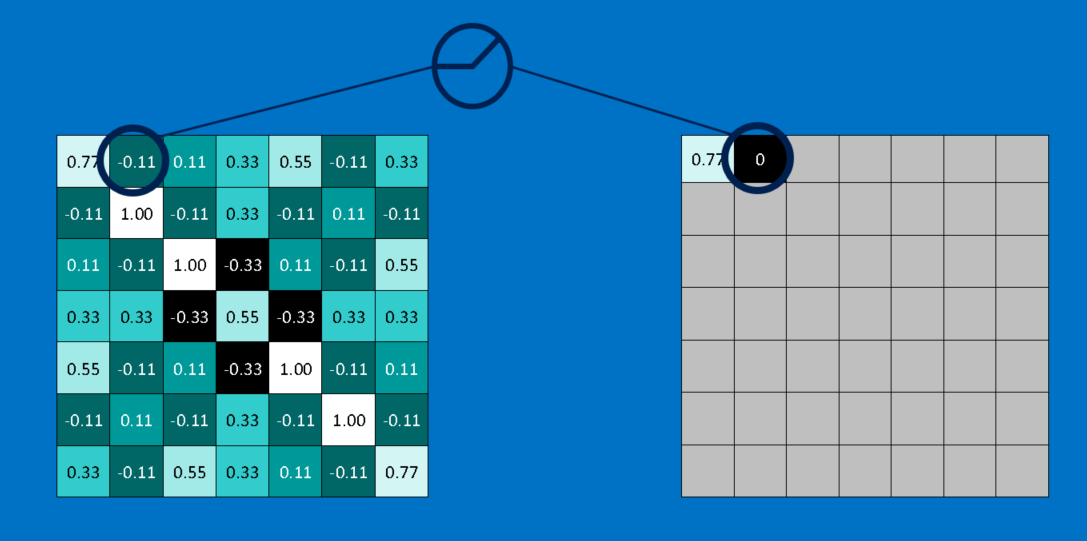
\includegraphics[scale=0.45]{RLU}
	\end{figure}

	В итоге все выглядит примерно так:
	Несколько чередующихся слоев свертки и подвыборки, разбавленные нормировкой ReLU и в конце обычный перцептрон.
	\\
	\\
	\\

	\begin{figure}[h!]
		
		\centering
		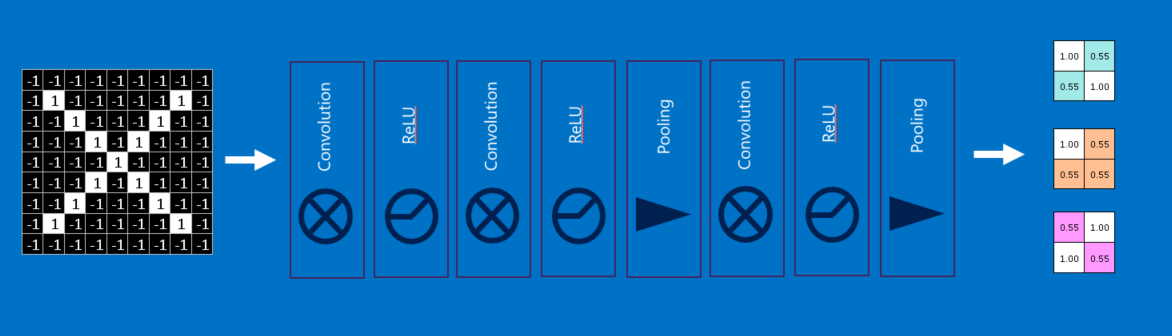
\includegraphics[scale=0.5]{all_step}
	\end{figure}
	
	\begin{figure}[h!]
		\centering
		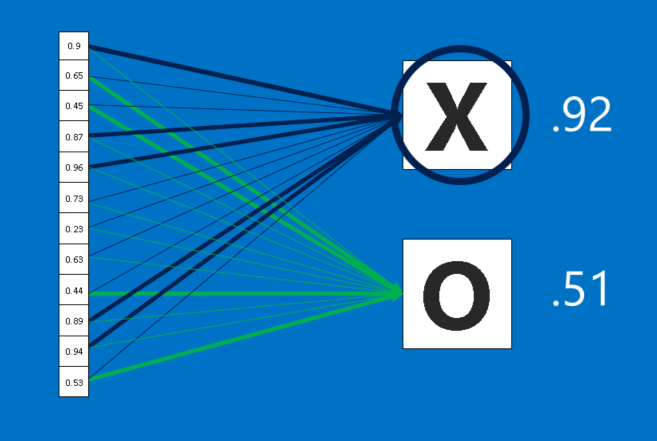
\includegraphics[scale=0.45]{final}
	\end{figure}


	%----------------------------------------------------------------------------------------
	%	PROBLEM 9
	%----------------------------------------------------------------------------------------
	\section{Рекуррентные нейронные сети}
	Свёрточные слои хорошо подходят для анализа изображений, поскольку учитывают их пространственную структуру. Текстовые данные представляют собой последовательный набор токенов (то есть символов, букв или других базовых элементов), и для работы с ними применяются рекуррентные сети (recurrent neural networks), позволяющие обрабатывать такие последовательности. В рекуррентных слоях дополнительно появляется время — в каждый следующий момент времени t на вход подаётся очередной токен $x_t$ из входной последовательности. Также рекуррентный слой хранит скрытое состояние $h_t$, которое позволяет «помнить» токены, которые поступали на вход ранее.


	\begin{figure}[h!]
		\centering
		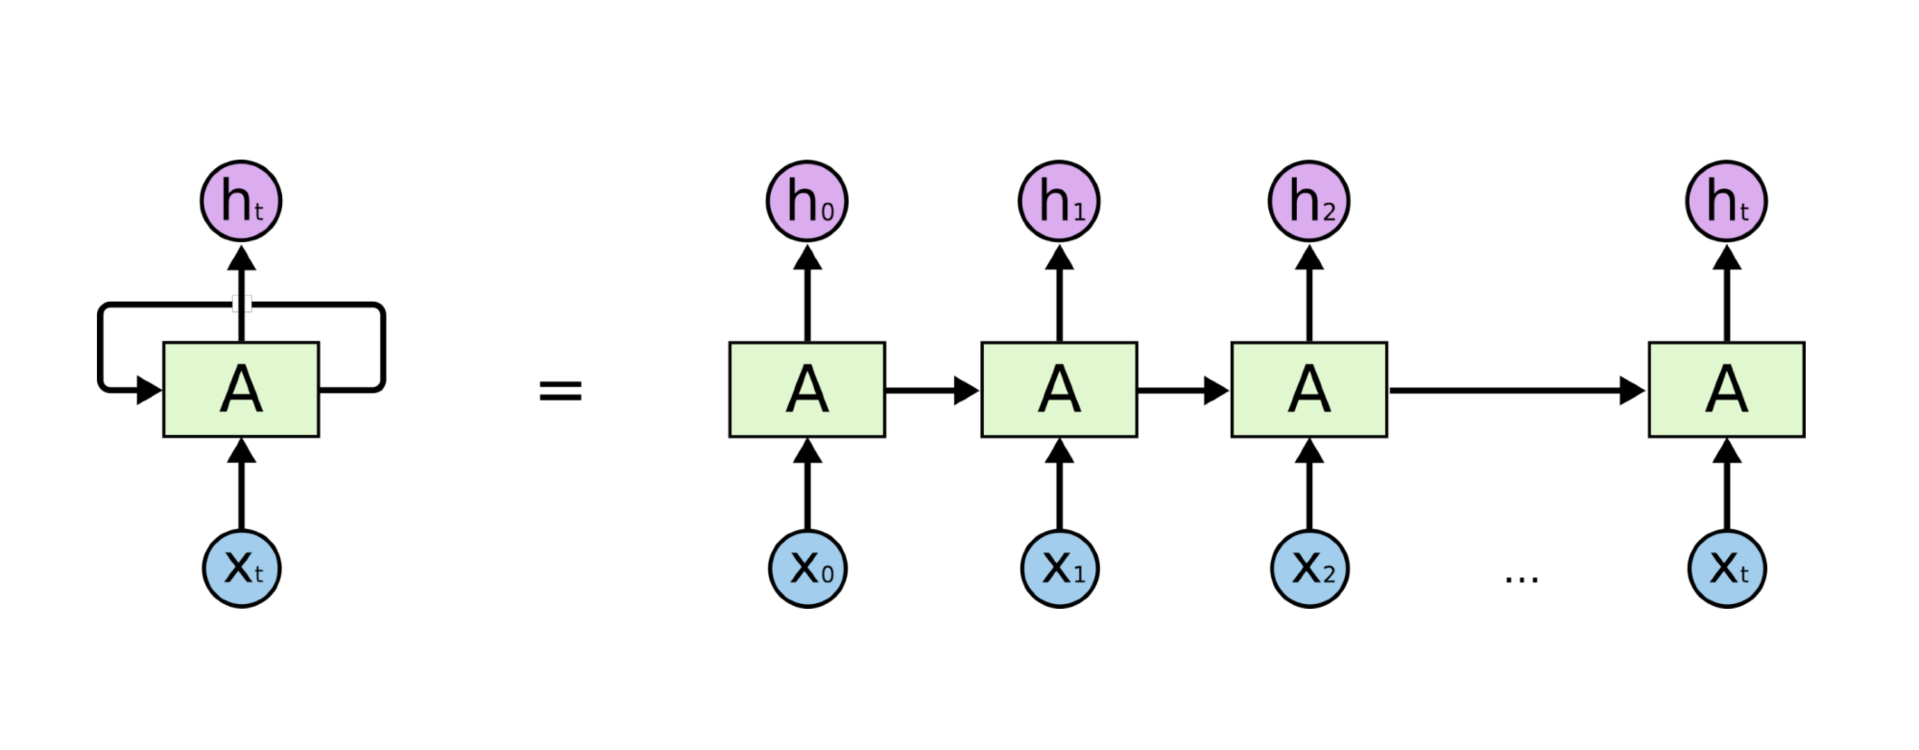
\includegraphics[scale=0.24]{recurent}
	\end{figure}


	\begin{figure}[h!]
		\centering
		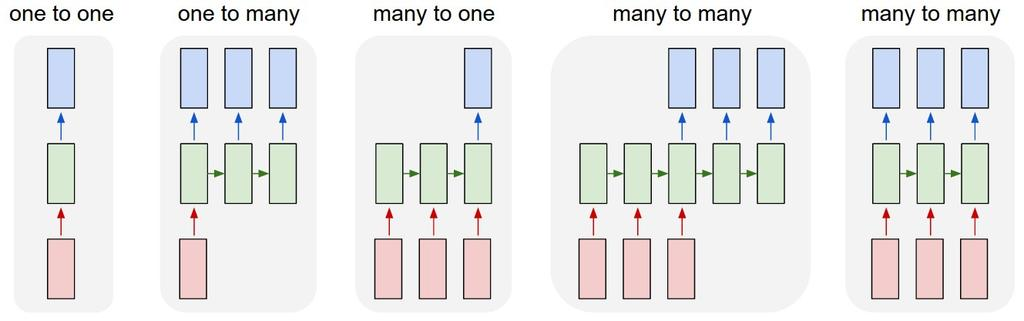
\includegraphics[scale=0.45]{recurr_type}
	\end{figure}

	
	
	\begin{enumerate}
	\item $ONE-TO-ONE$ Это обычная сеть прямого распространения. Картинка на вход, класс на выход. 
	
	Дальше идут рекуррентные типы.
	
	\item $ONE-TO-MANY$ подходит для аннотирования изображений. Т.е. картинка на вход, предложение на выход.
	\item $MANY-TO-ONE$ используется для классификации текста. (например хороший/плохой отзыв). Слова на входе и оценка на выходе.
	\item $MANY-TO-MANY$ дает нам машинный перевод. Предложение на вход, предложение на выход. Или же вопрос-ответная система. 
	и наконец
	\item $MANY-TO-MANY$ используется для классификации видео. Видео на вход, описание на выход.

	\end{enumerate}
	
	%----------------------------------------------------------------------------------------
	%	PROBLEM 10
	%----------------------------------------------------------------------------------------
	\section{Сети с долгой краткосрочной памятью (LSTM)}
	LSTM это все те же рекуррентные сети, но с некоторой добавкой. Тут меняется архитектура так, что бы сеть могла запоминать данные на значительно более долгое время. Основной элемент данной сети, это специального вида нейрон, который используется в качестве ячейки памяти(memory cell).
	
	\begin{figure}[h!]
		\centering
		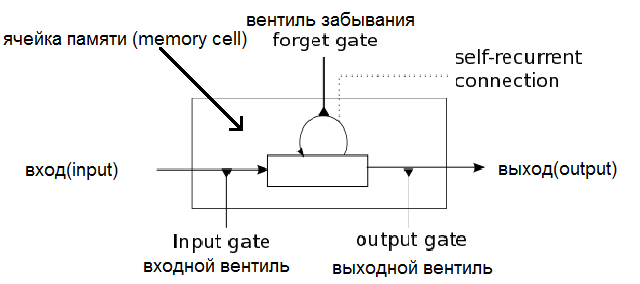
\includegraphics[scale=0.75]{mem_cell}
	\end{figure}
	
	Данный нейрон состоит из:
	
	\begin{enumerate}
	\item Вход сети (input)
	\item Выход сети (output)
	\item Память или состояние сети (memory cell)
	\item Блок очистки памяти (forget gate).
	\item Блок обновления памяти (input gate).
	\item Блок выдачи результата (output gate).
	\end{enumerate}
	
	Вес рекуррентной связи (self-recurrent connection) выставляется в 1. Таким образом, если ничего другого не происходит, то на каждом этапе значение переписывается, что и дает сохранение памяти. Для управления таким нейронном используется 3 вентиля: входной, выходной и забывания. Они регулируются другими нейронами сети. \\
	Рассмотрим как это работает немного подробнее.  \\
	Пусть на вход подается какое-то число. Тогда чтобы сохранить его значение необходимо выставить значение входного вентиля в единицу. Тогда значение запишется в ячейку памяти. Чтобы при поступлении следующих данных наше значение сохранилось "закрываем" вентиль, выставляя значение 0. Если хотим получить сохраненное значение на выход, то выставляем выходной вентиль в единицу.  \\
	Когда значение нам больше не требуется, можем его "забыть" выставив значение нейрона забывания в 0. После этого значение в нейроне очистится и можно записывать следующее.
	
	
	%----------------------------------------------------------------------------------------
	%	PROBLEM 11
	%----------------------------------------------------------------------------------------
	\section{Метод опорных векторов (support vector machines, SVM)}
	
	Основная идея метода — перевод исходных векторов в пространство более высокой размерности и поиск разделяющей гиперплоскости с максимальным зазором в этом пространстве.
	
	Часто в алгоритмах машинного обучения возникает необходимость классифицировать данные. Каждый объект данных представляется как вектор (точка) в $p-$мерном пространстве (упорядоченный набор $p$ чисел). Каждая из этих точек принадлежит только одному из двух классов. Вопрос состоит в том, можно ли разделить точки гиперплоскостью размерности ( $p-1$). Это - типичный случай линейной разделимости. Искомых гиперплоскостей может быть много, поэтому полагают, что максимизация зазора между классами способствует более уверенной классификации. То есть, можно ли найти такую гиперплоскость, чтобы расстояние от неё до ближайшей точки было максимальным. Это эквивалентно тому, что сумма расстояний до гиперплоскости от двух ближайших к ней точек, лежащих по разные стороны от нее, максимально. Если такая гиперплоскость существует, она называется \textbf{оптимальной разделяющей гиперплоскостью}, а соответствующий ей линейный классификатор называется \textbf{оптимально разделяющим классификатором}. \\
	Вектора, лежащие ближе всех к разделяющей гиперплоскости, называются опорными векторами (support vectors)
	
	\subsection{Немного математики}
	
	Пусть имеется обучающая выборка: $(x_1,y_1),\ldots,(x_m,y_m), x_i \in \mathbf{R^n}, y_i \in \{-1,1\}$
	Метод опорных векторов строит классифицирующую функцию $F$ в виде $$F(x) = sign(<w,x>+b),$$
	
	где $<,>$ - скалярное произведение, $w$ - нормальный вектор к разделяющей гиперплоскости,$b$ - вспомогательный параметр. Те объекты, для которых $F(x) = 1$ попадают в один класс, а объекты с $F(x) = -1$ - в другой.\\
	Выбор именно такой функции неслучаен: любая гиперплоскость может быть задана в виде $<w,x>+b$ для некоторых $w$ и $b$.
	
	Далее, мы хотим выбрать такие $a$ и $b$ которые максимизируют расстояние до каждого класса. 
	\\
	\\
	\\
	\\
	\begin{figure}[h!]
		\centering
		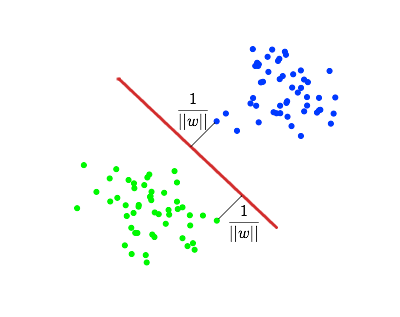
\includegraphics[scale=0.75]{svm}
	\end{figure}
	
	На практике случаи, когда данные можно разделить гиперплоскостью, или, как еще говорят, линейно, довольно редки.
	\begin{figure}[h!]
		\centering
		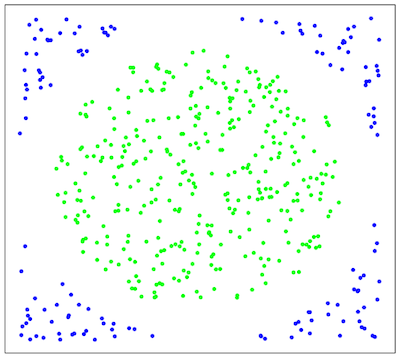
\includegraphics[scale=0.45]{svm2}
	\end{figure}

	В этом случае поступают так: все элементы обучающей выборки вкладываются в пространство X более высокой размерности с помощью специального отображения $\varphi : \mathbf{R^n} \longrightarrow X$. При этом отображение $\varphi$ выбирается так, чтобы в новом пространстве $X$ выборка была линейно разделима.
	
	Суть в том, что нам не обязательно делать отображение явным, т.к. в SVM фигурирует только скалярное произведение вектора весов на вектор признаков. Вместо этого использовать, возможно нелинейную, функцию $K(w,x) = <\varphi(w), \varphi(x)>$ и таким образом получать нелинейную разделяющую поверхность. $K-$ называется ядром классификатора.
	
	\begin{figure}[h!]
		\centering
		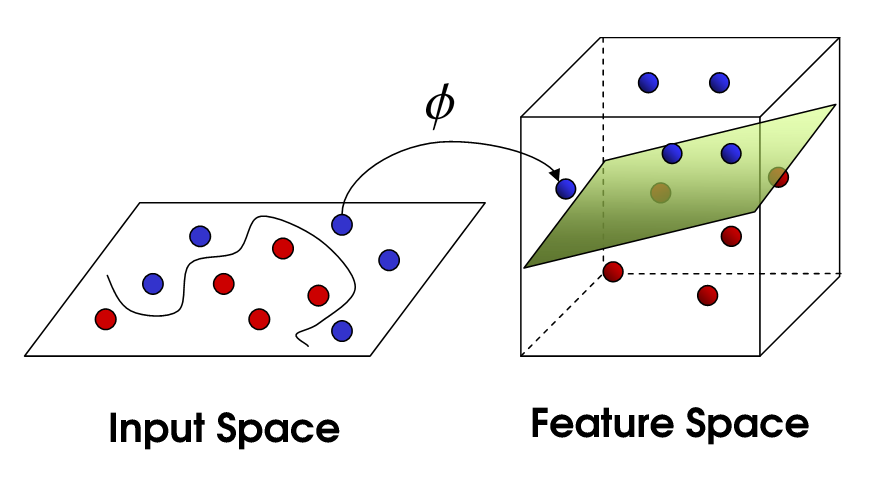
\includegraphics[scale=0.35]{kernal1}
	\end{figure}

	Есть несколько видов ядер.\\
	
	Линейное - очевидно. Это наша прямая на плоскости. $K(w,x) = <w,x>$
	
	Другое ядро - полиномиальное. Отображает в пространство, где добавляются разные произведения и степени признаков. $K(w,x) = (\gamma <w,x> + r)^d$
	
	Радиальное ядро - $K(w,x) = e^{-\gamma \|w - x\|^2}$
	
	%----------------------------------------------------------------------------------------
	%	PROBLEM 12
	%----------------------------------------------------------------------------------------
	\section{Нейронные сети Кохонена}
	Нейронные сети Кохонена типичный пример нейросетевой архитектуры, обучающейся без учителя. Отсюда и перечень решаемых ими задач: кластеризация данных или прогнозирование свойств. Кроме того, сети Кохонена могут использоваться с целью уменьшения размерности данных с минимальной потерей информации.
	
	\begin{figure}[h!]
		\centering
		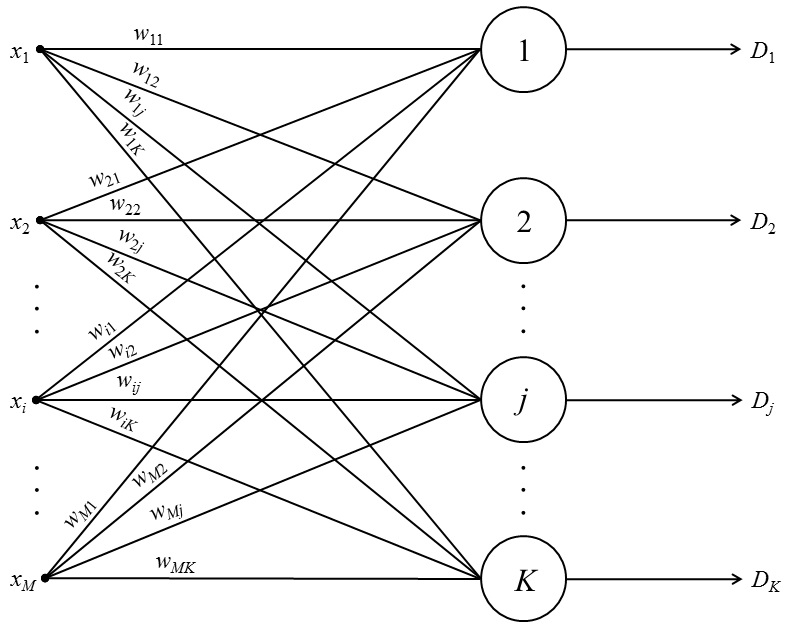
\includegraphics[scale=0.35]{koh}
	\end{figure}
	
	Количество нейронов равно количеству кластеров, среди которых происходит начальное распределение и последующее перераспределение обучающих примеров. Количество входных переменных нейронной сети равно числу признаков, характеризующих объект исследования и на основе которых происходит отнесение его к одному из кластеров.
	
	Следует различать собственно самообучение и самоорганизацию нейронной сети Кохонена. При обычном самообучении сеть имеет строго фиксированную структуру, т. е. количество нейронов, не изменяющееся на протяжении всего жизненного цикла. При самоорганизации сеть, напротив, не имеет постоянной структуры. В зависимости от найденного расстояния до нейрона-победителя либо этот нейрон используется для кластеризации примера, либо для поданного на входы примера создается новый кластер с соответствующими ему весовыми коэффициентами. Кроме того, в процессе самоорганизации структуры сети Кохонена отдельные нейроны могут исключаться из нее.

	Алгоритм обучения сети Кохонена включает этапы, состав которых зависит от типа структуры: постоянной (самообучающаяся сеть) или переменной (самоорганизующаяся сеть). Для самообучения последовательно выполняются:
	
	\begin{enumerate}
		\item Задание структуры сети (количества нейронов слоя Кохонена) (K)
		\item Случайная инициализация весовых коэффициентов значениями, удовлетворяющими одному из следующих ограничений:
		\begin{enumerate}
			\item при нормализации исходной выборки в пределах [–1, 1]
			\item при нормализации исходной выборки в пределах [0, 1]
		\end{enumerate}
		\item Подача на входы сети случайного обучающего примера текущей эпохи обучения и расчет евклидовых расстояний от входного вектора до центров всех кластеров 
		\begin{equation}
			R_j = \sqrt{\sum_{i = 1}^{M}(x_i - w_{ij})^2}
			\label{R}
		\end{equation}
		\item По наименьшему из значений $R_j$ выбирается нейрон-победитель $j$, в наибольшей степени близкий по значениям с входным вектором. Для выбранного нейрона (и только для него) выполняется коррекция весовых коэффициентов
		\item Цикл повторяется с шага 3 до выполнения одного или нескольких условий окончания:
		\begin{enumerate}
			\item исчерпано заданное предельное количество эпох обучения;
			\item не произошло значимого изменения весовых коэффициентов в пределах заданной точности на протяжении последней эпохи обучения;
			\item исчерпано заданное предельное физическое время обучения.
		\end{enumerate}
	\end{enumerate}

	В случае самоорганизации сети Кохонена алгоритм претерпевает определенные изменения:
	
	\begin{enumerate}
		\item Задается критическое расстояние $R_{кр}$, соответствующее максимально допустимому евклидову расстоянию между входами примера и весами нейрона-победителя. Начальная структура не содержит нейронов. При подаче на входы сети самого первого примера обучающей выборки создается первый нейрон с весовыми коэффициентами, равными поданным входным значениям.
		\item На входы сети подается новый случайно выбранный пример текущей эпохи обучения, рассчитываются евклидовы расстояния от примера до центра каждого кластера по соотношению $\ref{R}$ и определяется нейрон-победитель с наименьшим из них $R_{min}$.
		\item Если выполняется условие $R_{min} \le R_{кр}$, производится коррекция весовых коэффициентов соответствующего нейрона-победителя, в противном случае в структуру сети добавляется новый нейрон, весовые коэффициенты которого принимаются численно равными входным значениям поданного примера.
		\item Процедура повторяется с п.2. Если на протяжении последней эпохи обучения какие-либо кластеры остались не задействованными, соответствующие нейроны исключаются из структуры сети Кохонена.
		\item Вычисления заканчиваются, если выполняется одно из условий, прописанных в алгоритме самообучения сети фиксированной структуры.
	\end{enumerate}


	\section{BackPropagation }
	Небольшое напоминание об Методе обратного распространения ошибки. Т.к. он используется почти во всех сетях, то повторим и его, но коротенечко. \\
	Алгоритм обратного распространения ошибки следующий:
	
	\begin{enumerate}
		\item Инициализировать синаптические веса маленькими случайными значениями.
		\item Выбрать очередную обучающую пару из обучающего множества; подать входной вектор на вход сети.
		\item Вычислить выход сети.
		\item Вычислить разность между выходом сети и требуемым выходом 
		\item Подкорректировать веса сети для минимизации ошибки 
		\item Повторять шаги с 2 по 5 для каждого вектора обучающего множества до тех пор, пока ошибка на всем множестве не достигнет приемлемого уровня.
	\end{enumerate}

	Теперь немного в более серьезном виде.
	\textbf{Алгоритм: BackPropagation ($\eta, \alpha, \{x^d_i, t^d\}^{n,m}_{i=1,d=1}, steps$)}

	\begin{enumerate}
		\item Инициализировать $\{w_{ij}\}_{i,j}$  маленькими случайными значениями, $\{\Delta w_{ij}\}_{i,j} = 0$.
		\item Повторить NUMBER\_OF\_STEPS раз:\\
		Для всех d от 1 до m:
		\begin{enumerate}
			\item Подать ${x_i^d}$ на вход сети и подсчитать выходы $o_i$ каждого узла.
			\item Для всех $k \in Outputs$.
			$$\delta_k = o_k(1-o_k)(t_k-o_k)$$
			\item Для каждого уровня l, начиная с предпоследнего:\\
			Для каждого узла j уровня l вычислить
			$$\delta_j = o_j(1-o_j) \sum_{k \in Children(j)} \delta_k w_{j,k}$$
			\item Для каждого ребра сети $\{i, j\}$
			$$\Delta w_{i,j}(n) = \alpha \Delta w_{i,j} (n-1) + (1-\alpha) \eta \delta_j o_i$$
			$$w_{i,j}(n) =w_{i,j} (n-1) + \Delta w_{i,j}(n)$$
		\end{enumerate}
	\item Выдать значения $w_{ij}$.
	\end{enumerate}
	Где $\alpha - $ коэффициент инерциальности для сглаживания резких скачков при перемещении по поверхности целевой функции.

\end{document}
